% !TEX TS-program = pdflatex
% !TEX encoding = UTF-8 Unicode


\documentclass[12pt]{article} 

\usepackage[utf8]{inputenc} % set input encoding. utf8 or greater 4 lyfe. 

%%% PAGE DIMENSIONS
\usepackage{geometry} % to change the page dimensions
\geometry{a4paper} 
%\geometry{margin=2in} % for example, change the margins to 2 inches all round
% \geometry{landscape} % set up the page for landscape
%   read geometry.pdf for detailed page layout information

\usepackage{graphicx} % support the \includegraphics command and options

% \usepackage[parfill]{parskip} % Activate to begin paragraphs with an empty line rather than an indent

%%% PACKAGES
\usepackage{booktabs} % for much better looking tables
\usepackage{array} % for better arrays (eg matrices) in maths
\usepackage{paralist} % very flexible & customisable lists (eg. enumerate/itemize, etc.)
\usepackage{verbatim} % adds environment for commenting out blocks of text & for better verbatim
\usepackage{subfig} % make it possible to include more than one captioned figure/table in a single float
% These packages are all incorporated in the memoir class to one degree or another...
\usepackage{listings} % for code segment environments.
% see http://en.wikibooks.org/wiki/LaTeX/Source_Code_Listings
\usepackage{tikz} % for FSM drawings from http://madebyevan.com/fsm/

%%% HEADERS & FOOTERS
\usepackage{fancyhdr} % This should be set AFTER setting up the page geometry
\pagestyle{fancy} % options: empty , plain , fancy
\renewcommand{\headrulewidth}{0pt} % customise the layout...
% headers
\lhead{TDT4205 Compiler Design, spring 2014}\chead{}\rhead{[trondrud]}
% footers
\lfoot{}\cfoot{\thepage}\rfoot{}

%%% SECTION TITLE APPEARANCE
\usepackage{sectsty}
% \allsectionsfont{\sffamily\mdseries\upshape} % (See the fntguide.pdf for font help)
% (This matches ConTeXt defaults)

%%% ToC (table of contents) APPEARANCE
\usepackage[nottoc,notlof,notlot]{tocbibind} % Put the bibliography in the ToC
\usepackage[titles,subfigure]{tocloft} % Alter the style of the Table of Contents
\renewcommand{\cftsecfont}{\rmfamily\mdseries\upshape}
\renewcommand{\cftsecpagefont}{\rmfamily\mdseries\upshape} % No bold!

\setcounter{secnumdepth}{0}

%%% END Article customizations

%%% The "real" document content comes below...

\title{Assignment 01, TDT4205}
\author{Odd M. Trondrud}
%\date{} % Activate to display a given date or no date (if empty),
         % otherwise the current date is printed 

\begin{document}
\maketitle

\part{Theory}
\section{Problem 1}
\begin{quote}
Try logging in to \texttt{login.stud.ntnu.no}. What version of gcc, flex and bison is installed on the server?
\end{quote}

\begin{verbatim}
$ gcc --version
gcc (Ubuntu/Linaro 4.6.3-1ubuntu5) 4.6.3
\end{verbatim}

\begin{verbatim}
$ flex --version
flex 2.5.35
\end{verbatim}

\begin{verbatim}
$ bison --version
$ bison (GNU Bison) 2.5
\end{verbatim}

\section{Problem 2}
\begin{quote}
What is the difference between an interpreter and a compiler?
\end{quote}

A compiler produces an executable from the source code that can be run on some architecture/system.
An interpreter performs the instructions in the source code as it is.
Python is an example of an interpreted language (the .py source files are can be run directly on a system with a python interpreter installed), while C is an example of a compiled language.
Java is weird.

\section{Problem 3}
\subsection{a)}
\begin{quote}
Construct a nondeterministic finite automaton for the language \texttt{10*10(0|1)*0}.
\end{quote}

Figure made with \texttt{http://madebyevan.com/fsm/}.

\begin{center}
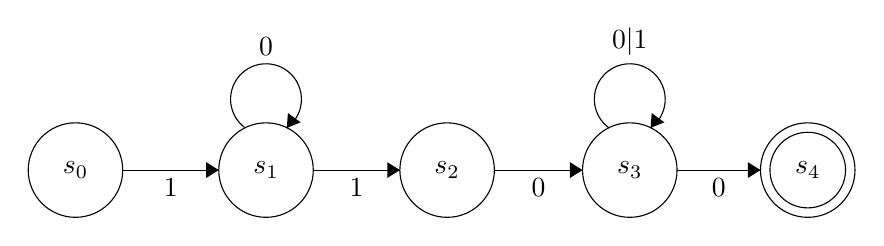
\begin{tikzpicture}[scale=0.2]
\tikzstyle{every node}+=[inner sep=0pt]
\draw [black] (21,-27.8) circle (3);
\draw (21,-27.8) node {$s_0$};
\draw [black] (33.1,-27.8) circle (3);
\draw (33.1,-27.8) node {$s_1$};
\draw [black] (44.6,-27.8) circle (3);
\draw (44.6,-27.8) node {$s_2$};
\draw [black] (56.2,-27.8) circle (3);
\draw (56.2,-27.8) node {$s_3$};
\draw [black] (67.5,-27.8) circle (3);
\draw (67.5,-27.8) node {$s_4$};
\draw [black] (67.5,-27.8) circle (2.4);
\draw [black] (24,-27.8) -- (30.1,-27.8);
\fill [black] (30.1,-27.8) -- (29.3,-27.3) -- (29.3,-28.3);
\draw (27.05,-28.3) node [below] {$1$};
\draw [black] (31.777,-25.12) arc (234:-54:2.25);
\draw (33.1,-20.55) node [above] {$0$};
\fill [black] (34.42,-25.12) -- (35.3,-24.77) -- (34.49,-24.18);
\draw [black] (36.1,-27.8) -- (41.6,-27.8);
\fill [black] (41.6,-27.8) -- (40.8,-27.3) -- (40.8,-28.3);
\draw (38.85,-28.3) node [below] {$1$};
\draw [black] (47.6,-27.8) -- (53.2,-27.8);
\fill [black] (53.2,-27.8) -- (52.4,-27.3) -- (52.4,-28.3);
\draw (50.4,-28.3) node [below] {$0$};
\draw [black] (54.877,-25.12) arc (234:-54:2.25);
\draw (56.2,-20.55) node [above] {$0|1$};
\fill [black] (57.52,-25.12) -- (58.4,-24.77) -- (57.59,-24.18);
\draw [black] (59.2,-27.8) -- (64.5,-27.8);
\fill [black] (64.5,-27.8) -- (63.7,-27.3) -- (63.7,-28.3);
\draw (61.85,-28.3) node [below] {$0$};
\end{tikzpicture}
\end{center}


\subsection{b)}
\begin{quote}
Describe what kind of words the language includes (with examples).
\end{quote}
The language includes words that begin with 1 followed by an arbitrary number of 0s, followed by 10, followed by an arbitrarily long combination of 0s and 1s followed by a 0.

\subsection{c)}
\begin{quote}
Create a transition table for the language, based on your automaton.
\end{quote}

\begin{center}

\begin{tabular}{c||cc}
	\hline \hline
	State & 0 & 1 \\ \hline
	$s_0$ & $\emptyset$ & $\{s_1\}$ \\
	$s_1$ & $\{s_1\}$ & $\{s_2\}$ \\
	$s_2$ & $\{s_3\}$ & $\emptyset$ \\
	$s_3$ & $\{s_3, s_4\}$ & $\{s_3\}$ \\
	$s_4$ & $\emptyset$ & $\emptyset$ \\ \hline
\end{tabular}

\end{center}

\section{Problem 4}


\end{document}
